\documentclass[12pt,a4paper]{extarticle}
\usepackage[left=3cm,right=1cm,
    top=2cm,bottom=2cm,bindingoffset=0cm]{geometry}
\usepackage[utf8]{inputenc}
\usepackage[russian]{babel}
\usepackage[OT1]{fontenc}
\usepackage{amsmath}
\usepackage{amsfonts}
\usepackage{amssymb}
\usepackage{graphicx}
\usepackage{listings}
\usepackage{here}
\usepackage{xcolor}
\usepackage{hyperref}
\graphicspath{{image/}}
\bibliographystyle{plain}

\lstdefinestyle{base_listing}{
  extendedchars     = {true},
  inputencoding     = {utf8}, 
  basicstyle        = {\ttfamily \scriptsize},
  keywordstyle      = {\rmfamily \bfseries},
  commentstyle      = {\rmfamily \itshape},
  tabsize           = {2},
  flexiblecolumns   = {false},
  frame             = {single},
  showstringspaces  = {false},
  breaklines        = {true}, 
  breakatwhitespace = {true}
}

\lstdefinelanguage{LLVM-asm}
{
  morekeywords = {
    load, store, malloc, alloca, free, getelementptr,
    add, sub, insertvalue, extractvalue, icmp, call,
    define, void, global
  },
  sensitive   = false,
  morecomment = [l]{;}
}

\lstdefinestyle{crs_llvm}{
  style    = {base_listing},
  language = {LLVM-asm}
}

\lstdefinestyle{crs_cpp}{
  style    = {base_listing},
  language = {C++}
}

\lstdefinestyle{crs_sql}{
  style    = {base_listing},
  language = {SQL}
}

\lstdefinestyle{crs_bash}{
  style    = {base_listing},
  language = {bash}
}

\lstdefinestyle{crs_python}{
  style    = {base_listing},
  language = {python}
}


\begin{document}
	\begin{titlepage}
		\begin{center}
			Санкт-Петербургский политехнический	университет Петра Великого\\
			Институт компьютерных наук и технологий\\
			Кафедра компьютерных систем и программных технологий\\
			\vspace{6cm}
			Отчет по лабораторной работе\\
			по дисциплине <<Параллельные вычисления>>\\
			\Large
			Параллельные программы на С++ с использованием\\
			Pthreads и MPI\\
			\small
		\end{center}
		\vspace{3cm}
		\begin{flushright}
			Выполнил студент группы 13541/4\\
			Абдуллин А. М.\\
			\vspace{1cm}			
			Преподаватель:\\
			Стручков И. В.\\
		\end{flushright}
		\vspace{4cm}
		\begin{center}
			Санкт-Петербург\\
			2017 г.\\
		\end{center}
	\end{titlepage}
	\newpage

%%%%%%%%%%%%%%%%%%%%%%%%%%%%%%%%%%%%%%%%%%%%%%%%%%%%%%%%%%%%%%%%%%%%%%%%%%%%%%%%%%%%%%%%%%%%%%%%%%%%%%
%%%%%%%%%%%%%%%%%%%%%%%%%%%%%%%%%%%%%%%%%%%%%%%%%%%%%%%%%%%%%%%%%%%%%%%%%%%%%%%%%%%%%%%%%%%%%%%%%%%%%%
\section{Цель работы}
Изучить основы создания параллельных программ на С++ с использованием библиотек pthreads и MPI. Написать параллельную программу, которая решает следующую задачу: определение площади набора кругов, заданных массивом с координатами центров и радиусами, методом Монте-Карло.

%%%%%%%%%%%%%%%%%%%%%%%%%%%%%%%%%%%%%%%%%%%%%%%%%%%%%%%%%%%%%%%%%%%%%%%%%%%%%%%%%%%%%%%%%%%%%%%%%%%%%%
%%%%%%%%%%%%%%%%%%%%%%%%%%%%%%%%%%%%%%%%%%%%%%%%%%%%%%%%%%%%%%%%%%%%%%%%%%%%%%%%%%%%%%%%%%%%%%%%%%%%%%
\section{Метод Монте-Карло}
Метод Монте-Карло --- это метод приблизительного вычисления площадей фигур. Предположим, что необходимо вычислить площадь сложной фигуры ($S_{fig}$), расположенной на некой плоскости (рис. \ref{fig:monteKarlo}). Ограничим данную фигуру другой фигурой, площадь которой ($S_{total}$) легко вычисляется (например прямоугольник).
\begin{figure}[h!]
\center{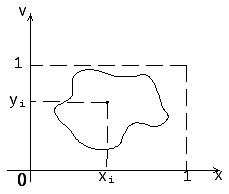
\includegraphics[scale=1]{monteKarlo}}
\caption{Метод Монте-Карло}
\label{fig:monteKarlo}
\end{figure}

Сгенерируем $N_{total}$ случайных точек, принадлежащих ограничивающей фигуре. Из этого набора случайных точек определим количество точек $N_{fig}$, который лежат в оригинальной фигуре. Таким образом получим следующую пропорцию:
\begin{equation*}
\frac{N_{fig}}{N_{total}} = \frac{S_{fig}}{S_{total}}
\end{equation*}

Отсюда можем оценить искомую площадь сложной фигуры:
\begin{equation*}
S_{fig} = \frac{N_{fig}}{N_{total}} * S_{total}
\end{equation*}

При этом чем больше точек $N_{total}$ будет проверено, тем точнее будет оценка площади.

%%%%%%%%%%%%%%%%%%%%%%%%%%%%%%%%%%%%%%%%%%%%%%%%%%%%%%%%%%%%%%%%%%%%%%%%%%%%%%%%%%%%%%%%%%%%%%%%%%%%%%
%%%%%%%%%%%%%%%%%%%%%%%%%%%%%%%%%%%%%%%%%%%%%%%%%%%%%%%%%%%%%%%%%%%%%%%%%%%%%%%%%%%%%%%%%%%%%%%%%%%%%%
\section{Однопоточная программа}

Для решения поставленной задачи была написана программа на С++. Программа принимает два входных аргумента:
\begin{itemize}
\item Путь к файлу с входными данными. В каждой строчке этого файла три числа: $x y r$, где $x$ -- абсцисса центра круга, $y$ -- ордината центра круга, $r$ -- радиус круга.
\item Число случайно генерируемых точек. 
\end{itemize}

Исходный код программы:
\begin{lstlisting}[caption={Однопоточная программа}, label={lst:prog1}, style=crs_cpp]
#include <iostream>
#include <fstream>
#include <limits>
#include <random>
#include <string>
#include <vector>

#include "Timer.h"

struct circle {
    double x;
    double y;
    double r;
};

double minx = std::numeric_limits<double>::max();
double miny = std::numeric_limits<double>::max();
double maxx = std::numeric_limits<double>::min();
double maxy = std::numeric_limits<double>::min();
std::vector<circle> circles;

bool inCircles(double x, double y) {
    for (auto it : circles) {
        auto dx = std::abs(x - it.x);
        auto dy = std::abs(y - it.y);
        if (dx * dx + dy * dy - it.r * it.r < 0) return true;
    }
    return false;
}


int thread(int numRepeats) {
    std::random_device r;
    std::default_random_engine re(r());
    std::uniform_real_distribution<double> xrand(minx, maxx);
    std::uniform_real_distribution<double> yrand(miny, maxy);
    int countIn = 0;
    for (auto i = 0; i < numRepeats; ++i) {
        double x = xrand(re);
        double y = yrand(re);
        if (inCircles(x, y)) ++countIn;
    }
    return countIn;
}

int main(int argc, char** argv) {
    if (argc < 2) {
        std::cout << "Usage: ./parallel *input file* *num dots*" << std::endl;
        return -1;
    }
    std::string inpFile = std::string(argv[1]);
    int numDots = atoi(argv[2]);

    if (numDots < 1) {
        std::cout << "Num dots and num threads must be bigger than 0" << std::endl;
        return -1;
    }

    double x, y, r;
    std::ifstream in(inpFile);
    while (in >> x) {
        in >> y >> r;
        circles.push_back({x, y, r});
    }

    for (auto it : circles) {
        if (it.x - it.r < minx) minx = it.x - it.r;
        if (it.x + it.r > maxx) maxx = it.x + it.r;
        if (it.y - it.r < miny) miny = it.y - it.r;
        if (it.y + it.r > maxy) maxy = it.y + it.r;
    }

    Timer timer{};
    int numDotsIn = thread(numDots);
    auto elapsedTime = timer.elapsed();

    double squareArea = (maxx - minx) * (maxy - miny);
    std::cout << "Total generated dots: " << numDots << std::endl;
    std::cout << "Total dots in: " << numDotsIn << std::endl;
    std::cout << "Square area: " << squareArea << std::endl;
    std::cout << "Circles area: " << ((double) numDotsIn / numDots) * squareArea << std::endl;
    std::cout << "Elapsed time: " << elapsedTime << std::endl;

    return 0;
}
\end{lstlisting}

Функция \texttt{main} считывает входные аргументы, определяет координаты прямоугольника, который очерчивает все окружности и вызывает функцию \texttt{thread}. Эта функция генерирует указанное количество случайных точек (лежащих в прямоугольнике) и проверяет каждую из точек с помощью функции \texttt{inCircles}. Функция возвращает число точек, лежащих внутри окружностей (т.е. $N_{fig}$). Функция \texttt{inCircles} проходит по всем окружностям, и если точка лежит хотя бы в одной из них, возвращает \texttt{true}.

Так же в \texttt{main} измеряется время, затраченное на вычисление площади. Время считается с помощью класса \texttt{Timer}:
\begin{lstlisting}[caption={Класс Timer}, label={lst:timer}, style=crs_cpp]
class Timer
{
public:
    Timer() : beg_(clock_::now()) {}
    void reset() { beg_ = clock_::now(); }
    double elapsed() const {
        return std::chrono::duration_cast<second_>
                (clock_::now() - beg_).count(); }

private:
    typedef std::chrono::high_resolution_clock clock_;
    typedef std::chrono::duration<double, std::ratio<1> > second_;
    std::chrono::time_point<clock_> beg_;
};
\end{lstlisting}

Пример запуска:
\begin{lstlisting}[style=crs_bash]
kivi@kivi-VirtualBox:~/workspace/parallel/parallel-not$ ./parallel input1 1000000
Total generated dots: 1000000
Total dots in: 784522
Square area: 4
Circles area: 3.13809
Elapsed time: 0.423313
\end{lstlisting}

%%%%%%%%%%%%%%%%%%%%%%%%%%%%%%%%%%%%%%%%%%%%%%%%%%%%%%%%%%%%%%%%%%%%%%%%%%%%%%%%%%%%%%%%%%%%%%%%%%%%%%
%%%%%%%%%%%%%%%%%%%%%%%%%%%%%%%%%%%%%%%%%%%%%%%%%%%%%%%%%%%%%%%%%%%%%%%%%%%%%%%%%%%%%%%%%%%%%%%%%%%%%%
\section{Многопоточность на Pthreads}

POSIX Threads --- стандарт POSIX реализации потоков (нитей) выполнения. Стандарт POSIX.1c, Threads extensions (IEEE Std 1003.1c-1995) определяет API для управления потоками, их синхронизации и планирования.

Однопоточная программа была реализована таким образом, что непосредственно в процессе вычисления площади глобальные переменные никак не изменяются, к ним осуществляется доступ только на чтение. Исходный код однопоточной программы был изменен следующим образом:
\begin{lstlisting}[caption={Многопоточность на Pthreads}, label={lst:pthreads}, style=crs_cpp]
void* thread(void* arg) {
    auto numRepeats = *(int*)arg;
    std::random_device r;
    std::default_random_engine re(r());
    std::uniform_real_distribution<double> xrand(minx, maxx);
    std::uniform_real_distribution<double> yrand(miny, maxy);
    int countIn = 0;
    for (auto i = 0; i < numRepeats; ++i) {
        double x = xrand(re);
        double y = yrand(re);
        if (inCircles(x, y)) ++countIn;
    }
    pthread_exit((void*) countIn);
}

int main(int argc, char** argv) {
    if (argc < 4) {
        std::cout << "Usage: ./parallel *input file* *num threads* *num dots*" << std::endl;
        return -1;
    }
    std::string inpFile = std::string(argv[1]);
    auto numThreads = atoi(argv[2]);
    auto numDots = atoi(argv[3]);

    if (numDots < 1 || numThreads < 1) {
        std::cout << "Num dots and num threads must be bigger than 0" << std::endl;
        return -1;
    }
    if (numDots < numThreads) {
        std::cout << "Num dots must be more than num threads" << std::endl;
        return -1;
    }


    double x, y, r;
    std::ifstream in(inpFile);
    while (in >> x) {
        in >> y >> r;
        circles.push_back({x, y, r});
    }

    for (auto it : circles) {
        if (it.x - it.r < minx) minx = it.x - it.r;
        if (it.x + it.r > maxx) maxx = it.x + it.r;
        if (it.y - it.r < miny) miny = it.y - it.r;
        if (it.y + it.r > maxy) maxy = it.y + it.r;
    }


    int dotsPerThread = numDots / numThreads;
    pthread_t* threads = new pthread_t[numThreads];

    Timer timer{};
    for (auto i = 0; i < numThreads; ++i) {
        if (pthread_create(&threads[i], NULL, thread, &dotsPerThread)) {
            std::cout << "Cannot create thread" << std::endl;
            return -1;
        }
    }

    int numDotsIn = 0;
    int retVal = 0;

    for (auto i = 0; i < numThreads; ++i) {
        if (pthread_join(threads[i], (void**)&retVal)) {
            std::cout << "Cannot join thread" << std::endl;
            return -1;
        }

        numDotsIn += retVal;
    }
    delete[] threads;
    auto elapsedTime = timer.elapsed();

    double squareArea = (maxx - minx) * (maxy - miny);
    auto allDots = dotsPerThread * numThreads;
    std::cout << "Total generated dots: " << dotsPerThread * numThreads << std::endl;
    std::cout << "Total dots in: " << numDotsIn << std::endl;
    std::cout << "Square area: " << squareArea << std::endl;
    std::cout << "Circles area: " << ((double)numDotsIn / allDots) * squareArea << std::endl;
    std::cout << "Elapsed time: " << elapsedTime << std::endl;
    return 0;
}
\end{lstlisting}

Программа принимает три аргумента:
\begin{itemize}
\item Файл с входными данными
\item Количество генерируемых точек
\item Число потоков в программе
\end{itemize}

Для создания потока используется функция \texttt{pthread\_create}, для получения возвращаемого значения потока используется функция \texttt{pthread\_join}.

Пример запуска:
\begin{lstlisting}[style=crs_bash]
kivi@kivi-VirtualBox:~/workspace/parallel/parallel-pthread$ ./parallel input1 1000000 4
Total generated dots: 1000000
Total dots in: 784892
Square area: 4
Circles area: 3.13957
Elapsed time: 0.139572
\end{lstlisting}

%%%%%%%%%%%%%%%%%%%%%%%%%%%%%%%%%%%%%%%%%%%%%%%%%%%%%%%%%%%%%%%%%%%%%%%%%%%%%%%%%%%%%%%%%%%%%%%%%%%%%%
%%%%%%%%%%%%%%%%%%%%%%%%%%%%%%%%%%%%%%%%%%%%%%%%%%%%%%%%%%%%%%%%%%%%%%%%%%%%%%%%%%%%%%%%%%%%%%%%%%%%%%
\section{Многопоточность на MPI}

Message Passing Interface (MPI, интерфейс передачи сообщений) --- программный интерфейс (API) для передачи информации, который позволяет обмениваться сообщениями между процессами, выполняющими одну задачу. Базовым механизмом связи между MPI процессами является передача и приём сообщений. Сообщение несёт в себе передаваемые данные и информацию, позволяющую принимающей стороне осуществлять их выборочный приём. Для работы была использована библиотека OpenMPI. Исходный код однопоточной программы был изменен следующим образом:
\begin{lstlisting}[caption={Многопоточность на Pthreads}, label={lst:pthreads}, style=crs_cpp]
int thread(int numRepeats) {
    std::random_device r;
    std::default_random_engine re(r());
    std::uniform_real_distribution<double> xrand(minx, maxx);
    std::uniform_real_distribution<double> yrand(miny, maxy);
    int countIn = 0;
    for (auto i = 0; i < numRepeats; ++i) {
        double x = xrand(re);
        double y = yrand(re);
        if (inCircles(x, y)) ++countIn;
    }
    return countIn;
}

int main(int argc, char** argv) {
    if (argc < 3) {
        std::cout << "Usage: ./parallel *input file* *num dots*" << std::endl;
        return -1;
    }
    std::string inpFile = std::string(argv[1]);
    int numDots = atoi(argv[2]);

    if (numDots < 1) {
        std::cout << "Num dots and num threads must be bigger than 0" << std::endl;
        return -1;
    }

    double x, y, r;
    std::ifstream in(inpFile);
    while (in >> x) {
        in >> y >> r;
        circles.push_back({x, y, r});
    }

    for (auto it : circles) {
        if (it.x - it.r < minx) minx = it.x - it.r;
        if (it.x + it.r > maxx) maxx = it.x + it.r;
        if (it.y - it.r < miny) miny = it.y - it.r;
        if (it.y + it.r > maxy) maxy = it.y + it.r;
    }


    int numproc, rank;
    Timer timer{};
    MPI_Init(&argc, &argv);
    MPI_Comm_size(MPI_COMM_WORLD, &numproc);
    MPI_Comm_rank(MPI_COMM_WORLD, &rank);

    int dotsPerThread = numDots / numproc;
    int numDotsIn = 0, result;

    numDotsIn = thread(dotsPerThread);

    MPI_Reduce(&numDotsIn, &result, 1, MPI_INT, MPI_SUM, 0, MPI_COMM_WORLD);
    auto elapsedTime = timer.elapsed();


    if (rank == 0) {
        double squareArea = (maxx - minx) * (maxy - miny);
        auto allDots = dotsPerThread * numproc;
        std::cout << "Total generated dots: " << allDots << std::endl;
        std::cout << "Total dots in: " << result << std::endl;
        std::cout << "Square area: " << squareArea << std::endl;
        std::cout << "Circles area: " << ((double) result / allDots) * squareArea << std::endl;
        std::cout << "Elapsed time: " << elapsedTime << std::endl;
    }

    MPI_Finalize();
    return 0;
}
\end{lstlisting}

Для работы программы в MPI необходимо перед началом межпроцессного обмена вызвать функцию \texttt{MPI\_Init}, а в конце вызвать \texttt{MPI\_Finalize}. По-сути MPI запускает несколько копий одного и того же процесса, у них различаются только ранги. Ранг и количество процессов можно получить с помощью функций \texttt{MPI\_Comm\_rank} и \texttt{MPI\_Comm\_size}. Каждый процесс MPI запускает функцию \texttt{thread} с необходимым количеством точек. Результат работы этой функции сохраняется в переменную \texttt{numDotsIn}. Далее с помощью функции \texttt{MPI\_Reduce} значения данной переменной объединяются в другую переменную на процессе с указанным рангом. Объединения происходит по указанной операции. В данном случае результаты объединяются на процессе с рангом 0 в переменную \texttt{result} с помощью суммирования. Далее этот процесс выводит результаты в консоль.

Запуск MPI-программы производится с помощью утилиты \texttt{mpiexec}, которая запускает все необходимые процессы. В качестве аргументов данной утилиты можно указать количество запускаемых процессов и более специфичные параметры (например, количество процессов запускающихся на каждом узле ВС). Пример работы:
\begin{lstlisting}[style=crs_bash]
kivi@kivi-VirtualBox:~/workspace/parallel/parallel-mpi$ mpiexec -np 4 ./parallel input1 1000000
Total generated dots: 1000000
Total dots in: 785309
Square area: 4
Circles area: 3.14124
\end{lstlisting}

%%%%%%%%%%%%%%%%%%%%%%%%%%%%%%%%%%%%%%%%%%%%%%%%%%%%%%%%%%%%%%%%%%%%%%%%%%%%%%%%%%%%%%%%%%%%%%%%%%%%%%
%%%%%%%%%%%%%%%%%%%%%%%%%%%%%%%%%%%%%%%%%%%%%%%%%%%%%%%%%%%%%%%%%%%%%%%%%%%%%%%%%%%%%%%%%%%%%%%%%%%%%%

\section{Эксперименты}

Для проведения экспериментов по измерению производительности программ было создано три входных набора данных.
\begin{lstlisting}[caption={Набор данных 1}, label={lst:input1}, style=crs_cpp]
0 0 1
\end{lstlisting}

\begin{lstlisting}[caption={Набор данных 2}, label={lst:input1}, style=crs_cpp]
0 0 10
18 16 100
5 0.1 0.1
\end{lstlisting}

\begin{lstlisting}[caption={Набор данных 3}, label={lst:input1}, style=crs_cpp]
0 0 19
14 18.1 19
4.3 3.3 10.5
0.1 0.01 53
109 -10 78.9
17.5 -7 7
5 5 1.01
\end{lstlisting}

Каждая программа запускалась на каждом наборе входных данных при $N_{total} = 1000000$. Pthread и MPI версии запускались при этом в $1, 2, 4, 8$ потоков.
\begin{lstlisting}[caption={Скрипт запуска}, label={lst:script}, style=crs_python]
import sys
from subprocess import Popen, PIPE

# arguments
args = list(sys.argv)
if len(args) < 4:
	sys.exit("Usage: python testparallel.py *programm* *input file* *num repeats*")

programm = args[1]
inputFile = args[2]
numRepeats = int(args[3])

#run programm

allAreas = 0.0
for proc in [1, 2, 4, 8]:
	times = []
	for i in range(numRepeats):
		process = Popen([programm, inputFile, '1000000', str(proc)], stdout=PIPE)
		exit_code = process.wait()
		if exit_code != 0:
			sys.exit("Cannot run programm")

		for line in process.stdout:
			if 'Circles' in line:
				allAreas = allAreas + float(line.split()[-1])
			if 'Elapsed' in line:
				times.append(float(line.split()[-1]))

	av = sum(times) / numRepeats
	disp = 0.0
	for val in times:
		disp = disp + (val - av) ** 2
	if numRepeats == 1:
		disp = disp / numRepeats
	else:
		disp = disp / (numRepeats - 1)

	print("{} threads: average = {}, dispersion = {}".format(proc, av, disp))

print("Average area = {}".format(allAreas / (4 * numRepeats)))
\end{lstlisting}

Данный скрипт принимает путь к исполняемому файлу, путь к файлу с входными данными и число повторных запусков каждой программы. В результате он выводит оценки мат. ожидания и дисперсии времени работы программы для каждой конфигурации запуска. Оценки мат. ожидания и дисперсии вычисляются по следующим формулам:
\begin{equation*}
M=\frac{\sum_{i}{x_i}}{n}
\end{equation*}
\begin{equation*}
D=\frac{1}{n - 1} {\sum_{i}{(x_i - M)^2}}
\end{equation*}

Так же данный скрипт выводит вычисленную среднюю площадь фигуры.

Запуск каждой программы был повторен 100 раз. Результаты экспериментов вы можете видеть в таблицах \ref{tab:input1} -- \ref{tab:input3}. Красным цветом выделены наиболее эффективные результаты.

\begin{table}
\caption{Результаты на первом наборе данных}
\center{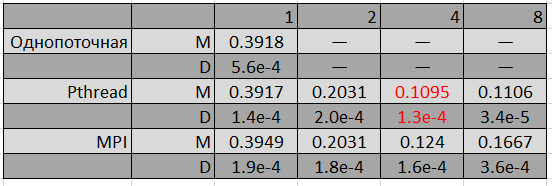
\includegraphics[scale=1]{input1}}
\label{tab:input1}
\end{table}

\begin{table}
\caption{Результаты на втором наборе данных}
\center{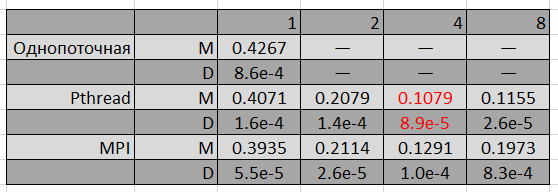
\includegraphics[scale=1]{input2}}
\label{tab:input2}
\end{table}

\begin{table}
\caption{Результаты на третьем наборе данных}
\center{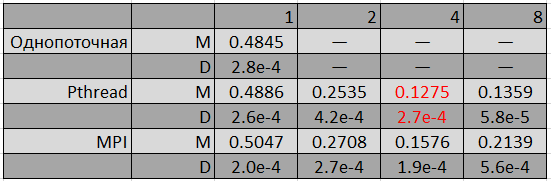
\includegraphics[scale=1]{input3}}
\label{tab:input3}
\end{table}

\section{Вывод}
В данной работе были изучены основы создания параллельных приложений на С++. Были изучены библиотеки Pthread и MPI. Созданные программы были протестированы на разных наборах данных и были оценены вероятностные характеристики времени работы.

На основе проведенных экспериментов можно сделать вывод, что наиболее эффективным решением является  решение на Pthread. Это достаточно неожиданный результат, так как MPI --- это стандарт, созданный специально для написания высокопараллельных программ. Можно предположить, что MPI оказался менее эффективен из-за того, что решаемая задача достаточно проста и примитивна, поэтому накладные расходы на синхронизацию процессов MPI оказываются слишком большими. В общем, можно сказать что MPI гораздо более предпочтителен для создания многопоточных программ, так как он обладает большим набором удобных функций и возможностей (например, широковещательная рассылка).

Программу удалось реализовать полностью независимой по данным, поэтому в работе не возникло необходимости использования средств синхронизации.

\end{document}